
\pdfminorversion=4 % for acroread
%\documentclass[aspectratio=169,t,xcolor={usenames,dvipsnames}]{beamer}
\documentclass[aspectratio=169,t,handout,xcolor={usenames,dvipsnames}]{beamer}
\usepackage{../beamerstyle}
\usepackage{dsfont}
\usepackage{bm}
\usepackage[english]{babel}
\usepackage[utf8]{inputenc}
\usepackage{graphicx}
\usepackage{algorithm}
\usepackage[ruled,vlined,algo2e,linesnumbered]{algorithm2e}
%\usepackage[boxed,vlined]{algorithm2e}
\usepackage{hyperref}
\usepackage{booktabs}
\usepackage{mathtools}

\usepackage{amsmath,amssymb}
\usepackage{listings}
\lstset{frame=lines,framesep=3pt,numbers=left,numberblanklines=false,basicstyle=\ttfamily\small}

\usepackage{subfig}
\usepackage{multicol}
%\usepackage{appendixnumberbeamer}
%
\usepackage{tcolorbox}

\usepackage{pgfplots}
\usepackage{tikz}
\usetikzlibrary{trees} 
\usetikzlibrary{shapes.geometric}
\usetikzlibrary{positioning,shapes,shadows,arrows,calc,mindmap}
\usetikzlibrary{positioning,fadings,through}
\usetikzlibrary{decorations.pathreplacing}
\usetikzlibrary{intersections}
\usetikzlibrary{positioning,fit,calc,shadows,backgrounds}
\pgfdeclarelayer{background}
\pgfdeclarelayer{foreground}
\pgfsetlayers{background,main,foreground}
\tikzstyle{activity}=[rectangle, draw=black, rounded corners, text centered, text width=8em]
\tikzstyle{data}=[rectangle, draw=black, text centered, text width=8em]
\tikzstyle{myarrow}=[->, thick, draw=black]

% Define the layers to draw the diagram
\pgfdeclarelayer{background}
\pgfdeclarelayer{foreground}
\pgfsetlayers{background,main,foreground}

%\usepackage{listings}
%\lstset{numbers=left,
%  showstringspaces=false,
%  frame={tb},
%  captionpos=b,
%  lineskip=0pt,
%  basicstyle=\ttfamily,
%%  extendedchars=true,
%  stepnumber=1,
%  numberstyle=\small,
%  xleftmargin=1em,
%  breaklines
%}

 
\definecolor{blue}{RGB}{0, 74, 153}

\usetheme{Boadilla}
%\useinnertheme{rectangles}
\usecolortheme{whale}
\setbeamercolor{alerted text}{fg=blue}
\useoutertheme{infolines}
\setbeamertemplate{navigation symbols}{\vspace{-5pt}} % to lower the logo
\setbeamercolor{date in head/foot}{bg=white} % blue
\setbeamercolor{date in head/foot}{fg=white}
\setbeamercolor{author  in head/foot}{bg=white} %blue
\setbeamercolor{title in head/foot}{bg=white} % blue
\setbeamercolor{title}{fg=white, bg=blue}
\setbeamercolor{block title}{fg=white,bg=blue}
\setbeamercolor{block body}{bg=blue!10}
\setbeamercolor{frametitle}{fg=white, bg=blue}
\setbeamercovered{invisible}

\makeatletter
\setbeamertemplate{footline}
{
  \leavevmode%
  \hbox{%
  \begin{beamercolorbox}[wd=.333333\paperwidth,ht=2.25ex,dp=1ex,center]{author in head/foot}%
%    \usebeamerfont{author in head/foot}\insertshortauthor
  \end{beamercolorbox}%
  \begin{beamercolorbox}[wd=.333333\paperwidth,ht=2.25ex,dp=1ex,center]{title in head/foot}%
    \usebeamerfont{title in head/foot}\insertshorttitle
  \end{beamercolorbox}%
  \begin{beamercolorbox}[wd=.333333\paperwidth,ht=2.25ex,dp=1ex,right]{date in head/foot}%
    \usebeamerfont{date in head/foot}\insertshortdate{}\hspace*{2em}
%    \insertframenumber\hspace*{2ex} 
  \end{beamercolorbox}}%
  \vskip0pt%
}
\makeatother

%\pgfdeclareimage[height=1.2cm]{automl}{images/logos/automl.png}
%\pgfdeclareimage[height=1.2cm]{freiburg}{images/logos/freiburg}

%\logo{\pgfuseimage{freiburg}}

\renewcommand{\comment}[1]{
	\noindent
	%\vspace{0.25cm}
	{\color{red}{\textbf{TODO:} #1}}
	%\vspace{0.25cm}
}
\newcommand{\notefh}[1]{\textcolor{red}{\textbf{FH:} #1}}
\renewcommand{\comment}[1]{}
\newcommand{\hide}[1]{}
\newcommand{\cemph}[2]{\emph{\textcolor{#1}{#2}}}

\newcommand{\lit}[1]{{\footnotesize\color{black!60}[#1]}}

\newcommand{\litw}[1]{{\footnotesize\color{blue!20}[#1]}}


\newcommand{\myframe}[2]{\begin{frame}[c]{#1}#2\end{frame}}
\newcommand{\myframetop}[2]{\begin{frame}{#1}#2\end{frame}}
\newcommand{\myit}[1]{\begin{itemize}#1\end{itemize}}
\newcommand{\myblock}[2]{\begin{block}{#1}#2\end{block}}


\newcommand{\votepurple}[1]{\textcolor{Purple}{$\bigstar$}}
\newcommand{\voteyellow}[1]{\textcolor{Goldenrod}{$\bigstar$}}
\newcommand{\voteblue}[1]{\textcolor{RoyalBlue}{$\bigstar$}}
\newcommand{\votepink}[1]{\textcolor{Pink}{$\bigstar$}}

\newcommand{\diff}{\mathop{}\!\mathrm{d}}
\newcommand{\refstyle}[1]{{\small{\textcolor{gray}{#1}}}}
\newcommand{\hands}[0]{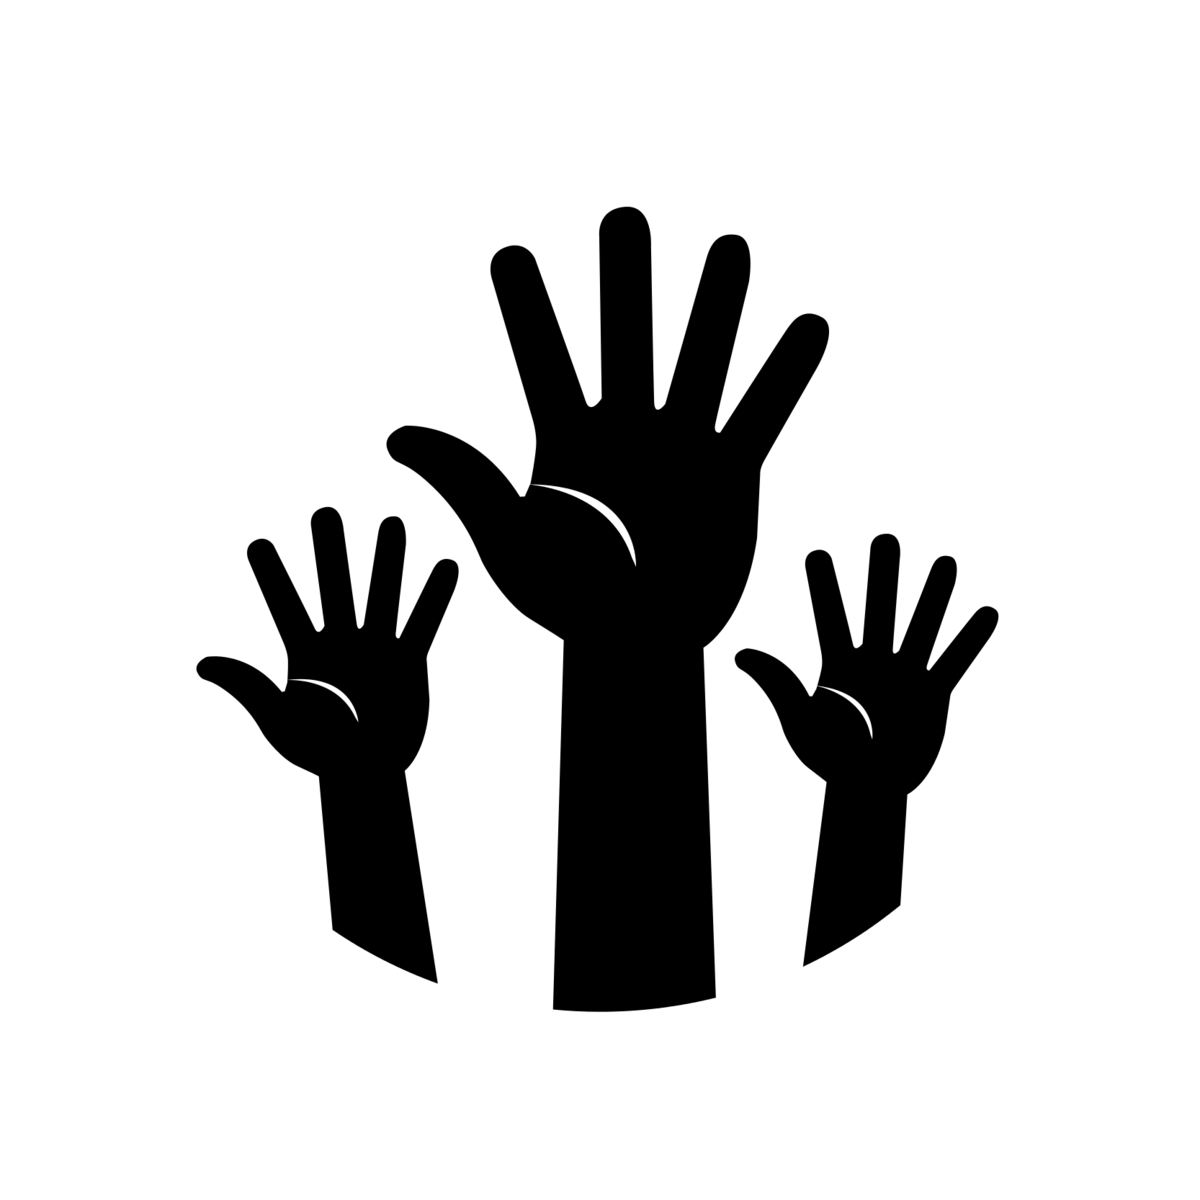
\includegraphics[height=1.5em]{images/hands}}
\newcommand{\transpose}[0]{{\textrm{\tiny{\sf{T}}}}}
\newcommand{\norm}{{\mathcal{N}}}
\newcommand{\cutoff}[0]{\kappa}
\newcommand{\instD}[0]{\dataset}
\newcommand{\insts}[0]{\mathcal{I}}
\newcommand{\inst}[0]{i}
\newcommand{\instI}[1]{i^{(#1)}}

% Iteration specific instance of variable/function/anything
% Introduced in the BO section, but moved up here to make it available within other macros
\newcommand{\iter}[2][\bocount]{{#2}^{(#1)}}

%--------HPO parameter macros-----------

% Parameter Configuration Space
\newcommand{\pcs}[0]{\pmb{\Lambda}}

% ???
\newcommand{\bx}[0]{\conf}

% Parameter Configuration
\newcommand{\conf}[0]{\pmb{\lambda}}

% Final Configuration
\newcommand{\finconf}[0]{\pmb{\hat{\lambda}}}

% Configuration corresponding to a given iteration -- better use \iter!
\newcommand{\confI}[1]{{\conf}^{(#1)}}

% Default Configuration
\newcommand{\defconf}[0]{{\conf}_{\text{def}}}

% Incumbent Configuration
\newcommand{\incumbent}[1][\bocount]{\iter[#1]{\finconf}}

% Optimal Configuration
\newcommand{\optconf}[0]{{\conf}^*}

% Configuration Space
\newcommand{\confs}[0]{\pcs}

%----------------------------------------

%\newcommand{\vlambda}[0]{\bm{\lambda}}
%\newcommand{\vLambda}[0]{\bm{\Lambda}}
\newcommand{\dataset}[0]{\mathcal{D}}
\newcommand{\datasets}[0]{\mathbf{D}}
\newcommand{\loss}[0]{L}
\newcommand{\risk}{\mathcal{R}}
\newcommand{\riske}{\mathcal{R}_{\text{emp}}}
\newcommand{\cost}[0]{c}
\newcommand{\costI}[1]{c^{(#1)}}

% Gaussian Process
\newcommand{\gp}{\mathcal{G}}
% Family of Objective Functions
\newcommand{\objF}{F}

%---------------BO Macros------------------

% BO loop counter
\newcommand{\bocount}{t}
% BO loop counter max, the counter runs from 1 to this value
\newcommand{\bobudget}{T}
% BO loop observation
\newcommand{\obs}[1][\conf]{\cost({#1})}
% BO loop observation space
\newcommand{\obsspace}{\mathcal{Y}}
% BO loop next observation
\newcommand{\bonextobs}{\obs[\iter{\conf}]}
% Acquisition Function, no args
\newcommand{\acq}{u}
% Standard Normal PDF
\newcommand{\pdf}{\phi}
% Standard Normal CDF
\newcommand{\cdf}{\Phi}
% Mean
\newcommand{\mean}{\mu}
% Standard Deviation
\newcommand{\stddev}{\sigma}
% Variance
\newcommand{\variance}{\sigma^2}
% Noise
\newcommand{\noise}{\nu}
% BO loop next selected sample
\newcommand{\bonextsample}{\confI{\bocount}}

% Single hyperparameter
\newcommand{\hyperparam}{\lambda}

% Single hyperparameter within a hyperparameter configuration
\newcommand{\hyperparami}[1][i]{{\hyperparam}_#1}

% Full definition of final configuration
\newcommand{\finconffull}{\incumbent[\bobudget]}

% Dataset
\newcommand{\datasetHPO}{{\dataset}_{HPO}}

% Dataset definition
\newcommand{\datasetHPOdef}{{\langle \bonextsample,\,\bonextobs \rangle}_{\bocount=1}^{\bobudget}}

% Double Display Fraction, forces large displays for everything in numerator and denominator
\newcommand\ddfrac[2]{\frac{\displaystyle #1}{\displaystyle #2}}

% Conditional Probability "Given That" Relation, source:https://tex.stackexchange.com/a/141685/205886
\newcommand\given[1][]{\:#1\vert\:}

% Expectation as a math operator
\DeclareMathOperator*{\E}{\mathbb{E}}

% Citation 
\newcommand{\source}[1]{
    \begin{flushright}
    	Source: \lit{#1}
    \end{flushright}
}
%-------------------------------------------

%Real numbers set
\newcommand{\realnum}{\mathbb{R}}
%Configuration space - do not use
%\newcommand{\configspace}{\Theta}
%Instances - do not use
%\newcommand{\instances}{\mathcal{I}}
%Expected value
\newcommand{\expectation}{\mathbb{E}}
%Kernel
\newcommand{\kernel}{\kappa}
%Constraint function
\newcommand{\constraintf}{c}
%Normal distribution
\newcommand{\normaldist}{\mathcal{N}}

% \renewcommand{\vec}[1]{\mathbf{#1}}
\newcommand{\hist}[0]{\dataset_{\text{Hist}}}
\newcommand{\param}[0]{p}
\newcommand{\algo}[0]{\mathcal{A}}
\newcommand{\algos}[0]{\mathbf{A}}
%\newcommand{\nn}[0]{N}
\newcommand{\feats}[0]{\mathcal{X}_{\text{meta}}}
\newcommand{\feat}[0]{\x_{\text{meta}}}
%\newcommand{\cluster}[0]{\vec{h}}
%\newcommand{\clusters}[0]{\vec{H}}
\newcommand{\perf}[0]{\mathbb{R}}
%\newcommand{\surro}[0]{\mathcal{S}}
\newcommand{\surro}[0]{\hat{\cost}}
\newcommand{\func}[0]{f}
\newcommand{\epm}[0]{\surro}
\newcommand{\portfolio}[0]{\mathbf{P}}
\newcommand{\schedule}[0]{\mathcal{S}}

% Machine Learning
\newcommand{\mdata}[0]{\dataset_{\text{meta}}}
\newcommand{\datasettrain}[0]{\dataset_{\text{train}}}
\newcommand{\datasetval}[0]{\dataset_{\text{val}}}
\newcommand{\datasettest}[0]{\dataset_{\text{test}}}
\newcommand{\x}[0]{\mathbf{x}}
\newcommand{\y}[0]{y}
\newcommand{\xI}[1]{\mathbf{x}^{(#1)}}
\newcommand{\yI}[1]{y^{(#1)}}
\newcommand{\fx}{f(\mathbf{x})}  % f(x), continuous prediction function
\newcommand{\Hspace}{\mathcal{H}} % hypothesis space where f is from
\newcommand{\fh}{\hat{f}}       % f hat, estimated prediction function

% Deep Learning
\newcommand{\weights}[0]{\theta}
\newcommand{\metaweights}[0]{\phi}


% reinforcement learning
\newcommand{\policies}[0]{\mathbf{\Pi}}
\newcommand{\policy}[0]{\pi}
\newcommand{\actionRL}[0]{a}
\newcommand{\stateRL}[0]{s}
\newcommand{\statesRL}[0]{\mathcal{S}}
\newcommand{\rewardRL}[0]{r}
\newcommand{\rewardfuncRL}[0]{\mathcal{R}}

\RestyleAlgo{algoruled}
\DontPrintSemicolon
\LinesNumbered
\SetAlgoVlined
\SetFuncSty{textsc}

\SetKwInOut{Input}{Input}
\SetKwInOut{Output}{Output}
\SetKw{Return}{return}

%\newcommand{\changed}[1]{{\color{red}#1}}

%\newcommand{\citeN}[1]{\citeauthor{#1}~(\citeyear{#1})}

\renewcommand{\vec}[1]{\mathbf{#1}}
\DeclareMathOperator*{\argmin}{arg\,min}
\DeclareMathOperator*{\argmax}{arg\,max}

%\newcommand{\aqme}{\textit{AQME}}
%\newcommand{\aslib}{\textit{ASlib}}
%\newcommand{\llama}{\textit{LLAMA}}
%\newcommand{\satzilla}{\textit{SATzilla}}
%\newcommand{\satzillaY}[1]{\textit{SATzilla'{#1}}}
%\newcommand{\snnap}{\textit{SNNAP}}
%\newcommand{\claspfolioTwo}{\textit{claspfolio~2}}
%\newcommand{\flexfolio}{\textit{FlexFolio}}
%\newcommand{\claspfolioOne}{\textit{claspfolio~1}}
%\newcommand{\isac}{\textit{ISAC}}
%\newcommand{\eisac}{\textit{EISAC}}
%\newcommand{\sss}{\textit{3S}}
%\newcommand{\sunny}{\textit{Sunny}}
%\newcommand{\ssspar}{\textit{3Spar}}
%\newcommand{\cshc}{\textit{CSHC}}
%\newcommand{\cshcpar}{\textit{CSHCpar}}
%\newcommand{\measp}{\textit{ME-ASP}}
%\newcommand{\aspeed}{\textit{aspeed}}
%\newcommand{\autofolio}{\textit{AutoFolio}}
%\newcommand{\cedalion}{\textit{Cedalion}}
\newcommand{\fanova}{\textit{fANOVA}}
\newcommand{\sbs}{\textit{SB}}
\newcommand{\oracle}{\textit{VBS}}

% like approaches
\newcommand{\claspfoliolike}[1]{\texttt{claspfolio-#1-like}}
\newcommand{\satzillalike}[1]{\texttt{SATzilla'#1-like}}
\newcommand{\isaclike}{\texttt{ISAC-like}}
\newcommand{\ssslike}{\texttt{3S-like}}
\newcommand{\measplike}{\texttt{ME-ASP-like}}

\newcommand{\irace}{\textit{I/F-race}}
\newcommand{\gga}{\textit{GGA}}
\newcommand{\smac}{\textit{SMAC}}
\newcommand{\paramils}{\textit{ParamILS}}
\newcommand{\spearmint}{\textit{Spearmint}}
\newcommand{\tpe}{\textit{TPE}}


\usepackage{pifont}
\newcommand{\itarrow}{\mbox{\Pisymbol{pzd}{229}}}
\newcommand{\ithook}{\mbox{\Pisymbol{pzd}{52}}}
\newcommand{\itcross}{\mbox{\Pisymbol{pzd}{56}}}
\newcommand{\ithand}{\mbox{\raisebox{-1pt}{\Pisymbol{pzd}{43}}}}

%\DeclareMathOperator*{\argmax}{arg\,max}

\newcommand{\ie}{{\it{}i.e.\/}}
\newcommand{\eg}{{\it{}e.g.\/}}
\newcommand{\cf}{{\it{}cf.\/}}
\newcommand{\wrt}{\mbox{w.r.t.}}
\newcommand{\vs}{{\it{}vs\/}}
\newcommand{\vsp}{{\it{}vs\/}}
\newcommand{\etc}{{\copyedit{etc.}}}
\newcommand{\etal}{{\it{}et al.\/}}

\newcommand{\pscProc}{{\bf procedure}}
\newcommand{\pscBegin}{{\bf begin}}
\newcommand{\pscEnd}{{\bf end}}
\newcommand{\pscEndIf}{{\bf endif}}
\newcommand{\pscFor}{{\bf for}}
\newcommand{\pscEach}{{\bf each}}
\newcommand{\pscThen}{{\bf then}}
\newcommand{\pscElse}{{\bf else}}
\newcommand{\pscWhile}{{\bf while}}
\newcommand{\pscIf}{{\bf if}}
\newcommand{\pscRepeat}{{\bf repeat}}
\newcommand{\pscUntil}{{\bf until}}
\newcommand{\pscWithProb}{{\bf with probability}}
\newcommand{\pscOtherwise}{{\bf otherwise}}
\newcommand{\pscDo}{{\bf do}}
\newcommand{\pscTo}{{\bf to}}
\newcommand{\pscOr}{{\bf or}}
\newcommand{\pscAnd}{{\bf and}}
\newcommand{\pscNot}{{\bf not}}
\newcommand{\pscFalse}{{\bf false}}
\newcommand{\pscEachElOf}{{\bf each element of}}
\newcommand{\pscReturn}{{\bf return}}

%\newcommand{\param}[1]{{\sl{}#1}}
\newcommand{\var}[1]{{\it{}#1}}
\newcommand{\cond}[1]{{\sf{}#1}}
%\newcommand{\state}[1]{{\sf{}#1}}
%\newcommand{\func}[1]{{\sl{}#1}}
\newcommand{\set}[1]{{\Bbb #1}}
%\newcommand{\inst}[1]{{\tt{}#1}}
\newcommand{\myurl}[1]{{\small\sf #1}}

\newcommand{\Nats}{{\Bbb N}}
\newcommand{\Reals}{{\Bbb R}}
\newcommand{\extset}[2]{\{#1 \; | \; #2\}}

\newcommand{\vbar}{$\,\;|$\hspace*{-1em}\raisebox{-0.3mm}{$\,\;\;|$}}
\newcommand{\vendbar}{\raisebox{+0.4mm}{$\,\;|$}}
\newcommand{\vend}{$\,\:\lfloor$}


\newcommand{\goleft}[2][.7]{\parbox[t]{#1\linewidth}{\strut\raggedright #2\strut}}
\newcommand{\rightimage}[2][.3]{\mbox{}\hfill\raisebox{1em-\height}[0pt][0pt]{\includegraphics[width=#1\linewidth]{#2}}\vspace*{-\baselineskip}}







\title[AutoML: DAC]{AutoML: Dynamic Configuration \& Learning}
\subtitle{Dynamic Configuration}
\author[Marius Lindauer]{Bernd Bischl \and Frank Hutter \and Lars Kotthoff\newline \and \underline{Marius Lindauer} \and Joaquin Vanschoren}
\institute{}
\date{}



% \AtBeginSection[] % Do nothing for \section*
% {
%   \begin{frame}{Outline}
%     \bigskip
%     \vfill
%     \tableofcontents[currentsection]
%   \end{frame}
% }

\begin{document}
	
	\maketitle
	

%----------------------------------------------------------------------
%----------------------------------------------------------------------
\begin{frame}[c]{Iterative Optimization Heuristics}
	
	\begin{itemize}
		\item Many iterative heuristics in algorithms are dynamic and adaptive
		\begin{enumerate}
			\item the algorithm's behavior changes over time
			\item the algorithm's behavior changes based on internal statistics
		\end{enumerate}
		\medskip
		\pause
		\item These heuristics might control other hyperparameters of the algorithms
		\pause
		\smallskip
		\item Example: learning rate schedules for training DNNs
		\begin{enumerate}
			\item exponential decaying learning rate: based on number of iterations, learning rate decreases
			\pause
			\item Reduce learning rate on plateaus: if the learning stagnates for some time,\\ the learning rate is decreased by a factor
		\end{enumerate}
		\pause
		\smallskip
		\item other examples: restart probability of search, mutation rate of evolutionary algorithms, \ldots  
		
	\end{itemize}
	
\end{frame}
%----------------------------------------------------------------------
%----------------------------------------------------------------------
\begin{frame}[c]{Parametrization of Learning Rate Schedules}
	
	\begin{itemize}
		\item How can we parameterize learning rate schedules?
		\begin{enumerate}
			\item exponential decaying learning rate:
			\begin{itemize}
				\item initial learning rate
				\item minimal learning rate
				\item multiplicative factor
			\end{itemize}
			\pause
			\item Reduce learning rate on plateaus:
			\begin{itemize}
				\item patience (in number of epochs)
				\item patience threshold
				\item decreasing factor
				\item cool-down break (in number of epochs)
			\end{itemize}
		\end{enumerate}
		\pause
		\medskip
		\item[$\leadsto$] Many hyperparameters only to control a single hyperparameter
		\pause   
		\item Still not guaranteed that optimal setting of e.g. learning rate schedules will lead to optimal learning behavior
		\begin{itemize}
			\item Learning rate schedules are only heuristics
		\end{itemize}
	\end{itemize}
	
\end{frame}
%----------------------------------------------------------------------
%----------------------------------------------------------------------
\begin{frame}[c]{Dynamic Algorithm Configuration}

\begin{itemize}
	\item So far, we assumed that an algorithm runs with static settings
	\item However, settings, such as learning rate, have to be adapted over time
\end{itemize}

\begin{block}{Definition}
	Let 
	\begin{itemize}
		\item $\conf \in \pcs$ be a hyperparameter configuration of an algorithm $\algo$,
		\pause
		\item $p(\dataset)$ be a probability distribution over meta datasets $\dataset \in \datasets$,
		\pause
		\item $\stateRL^{(t)}$ be a state description of $\algo$ solving $\dataset$ at time point $t$,
		\pause
		\item $\cost: \policies \times \datasets \to \perf$ be a cost metric assessing the cost of a control policy $\pi \in \Pi$ on $\dataset \in \datasets$
	\end{itemize}
	
	\pause
	the \emph{dynamic algorithm configuration problem} is to obtain a policy $\policy^* : \stateRL_t \times \dataset \mapsto \conf$ by optimizing its cost across a distribution of datasets:
	\begin{equation}
	\policy^* \in \argmin_{\policy \in \policies} \int_{\datasets} p(\dataset) \cost(\policy, \dataset) \diff \dataset \nonumber
	\end{equation}
\end{block}

\end{frame}
%-----------------------------------------------------------------------	

%----------------------------------------------------------------------
\begin{frame}[c]{Dynamic Algorithm Configuration as Contextual MDP \litw{\href{https://ml.informatik.uni-freiburg.de/papers/20-ECAI-DAC.pdf}{Biedenkapp et al. 2020}}}


\begin{description}
	\item[State $\stateRL^{(t)}$] are described by statistics gathered in the algorithm run
	\pause
	\item[Action $\actionRL^{(t)}$] change hyperparameters according to some control policy $\pi$
	\pause
	\item[Transition] run the algorithm from state $\stateRL^{(t)}$ to $\stateRL^{(t+1)}$ for a "short" moment by using the hyperparameters defined by $a^{(t)}$
	\pause
	\item[Reward $\rewardRL^{(t)}$] Return your current solution quality (or an approximation)
	\pause
	\item[Context $\dataset$] A given dataset (or task)
\end{description}

\bigskip
	
\centering
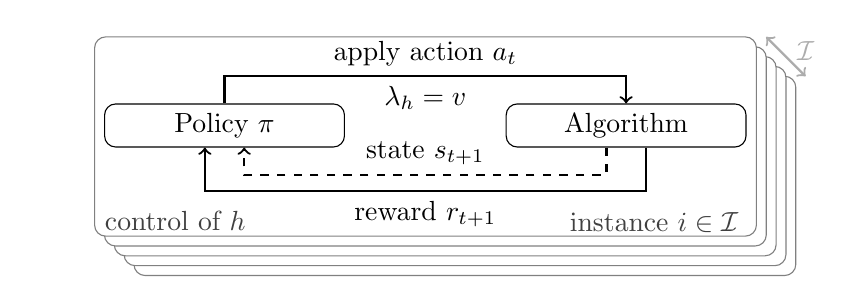
\begin{tikzpicture}[node distance=2.1cm]
        			%PreProcessing
        			
        			\node (Agent) [activity] {Policy $\policy$};
        			
        			\node (Algo) [activity, right of=Agent, xshift=3cm] {Algorithm};
        			
        			\begin{pgfonlayer}{background}
        			\path (Agent -| Agent.west)+(-0.12,1.125) node (resUL) {};
        			\path (Algo.east |- Algo.south)+(0.125,-1.125) node (resBR) {};
        			
        			% Context
        			\path [rounded corners, draw=black!50, fill=white] ($(resUL)+(0.5, -0.5)$) rectangle ($(resBR)+(0.5, -0.5)$);
        			\path [rounded corners, draw=black!50, fill=white] ($(resUL)+(0.375, -0.375)$) rectangle ($(resBR)+(0.375, -0.375)$);
        			\path [rounded corners, draw=black!50, fill=white] ($(resUL)+(0.25, -0.25)$) rectangle ($(resBR)+(0.25, -0.25)$);
        			\path [rounded corners, draw=black!50, fill=white] ($(resUL)+(0.125, -0.125)$) rectangle ($(resBR)+(0.125, -0.125)$);
        			
        			% Top level
        			\path [rounded corners, draw=black!50, fill=white] (resUL) rectangle (resBR);
        			\path (resBR)+(-1.3,0.175) node [text=black!75] {instance $\inst \in \insts$};
        			\path (resUL.east |- resBR.north)+(+.9,0.075) node [text=black!75] {control of $h$};
        			
        			\end{pgfonlayer}
        			
        			%        \draw[myarrow] (feat.south) -- ($(feat.south |- Agent)+(0,1.125)$);
        			
        			\draw[myarrow] (Agent.north) -- ($(Agent.north)+(0.0,+0.35)$) -- ($(Algo.north)+(0.0,+0.35)$) node [above,pos=0.5] {apply action $a_t$} node [below,pos=0.5] {$\lambda_h = v$} -- (Algo.north);
        			\draw[myarrow, dashed] ($(Algo.south)+(-0.25, 0)$) -- ($(Algo.south)+(-0.25, -0.35)$) -- ($(Agent.south)+(0.25, -0.35)$) node [above,pos=0.5] {state $s_{t+1}$} -- ($(Agent.south)+(0.25, 0)$);
        			\draw[myarrow] ($(Algo.south)+(0.25, 0)$) -- ($(Algo.south)+(0.25, -0.55)$) -- ($(Agent.south)+(-0.25, -0.55)$) node [below,pos=0.5] {reward $r_{t+1}$} -- ($(Agent.south)+(-0.25, 0)$);
        			
        			\draw[<->, thick, draw=black!32.5] (resBR.east |- resUL.center) -- ($(resBR.east |- resUL.center)+(0.5, -0.5)$);
        			\path (resBR.east |- resUL.center)+(.5, -0.175) node [text=black!32.5] {$\insts$};
        			% This path is only needed so the figure stays centered (the text is not visible)
        			\path (resUL.west |- resUL.center)+(-.5, -0.175) node [text=black!0] {$\insts$}; 
        			
        			\end{tikzpicture}
	
	
\end{frame}
%----------------------------------------------------------------------
%----------------------------------------------------------------------
\begin{frame}[c]{Solving Dynamic Algorithm Configuration}

Solve unknown MDP by using reinforcement learning (RL):

\begin{equation}
\mathcal{V}_\dataset^\policy(\stateRL^{(t)}) =  \mathbb{E} \left[\sum_{k=0}^\infty\gamma^k \rewardRL^{(t+k+1)}_\dataset| \stateRL^{(t)}=\stateRL \right]\nonumber
\end{equation}
\pause

\begin{equation}
 = \mathbb{E} \left[ \rewardRL^{(t+1)}_\dataset+\gamma\mathcal{V}_\dataset^\policy(\stateRL^{(t+1)})| \stateRL^{(t+1)} \sim \mathcal{T}_\dataset(\stateRL^{(t)}, \policy(\stateRL^{(t)})) \right] \nonumber
\end{equation}
\pause
\begin{equation}
\policy^* \in
\argmax_{\policy \in \policies}
\int_{\datasets} p(\dataset) \int_{\statesRL^{(0)}} \Pr(\stateRL^{(0)}) \cdot \mathcal{V}^\policy_\dataset(\stateRL^{(0)}) \diff \stateRL^{(0)} \diff \dataset \nonumber
\end{equation}

\bigskip
\pause
$\leadsto$ equivalent to Dynamic Algorithm Configuration definition


\end{frame}
%----------------------------------------------------------------------
%----------------------------------------------------------------------
\begin{frame}[c]{Dynamic Algorithm Configuration across Datasets \litw{\href{https://ml.informatik.uni-freiburg.de/papers/20-ECAI-DAC.pdf}{Biedenkapp et al. 2020}}}
	
\begin{itemize}
	\item Challenge: Evaluating a policies on all datasets is often not feasible
	\pause
	\item Curriculum learning \lit{Bengio et al. 2009} showed that we should have a curriculum of tasks we tackle
	\pause
	\item Self-paced learning \lit{Kumar et al. 2010} tries to automatically find such as a curriculum
	\begin{itemize}
		\item Focus on "easy" tasks where the agent can improve most:
	\end{itemize}
\end{itemize}
	
\pause
\begin{equation} 
\label{spl_loss}
\max_{\policy,\vec{v}}\mathcal{C}(\policy, \vec{v}, K) = \sum^{|\datasets|}_{i=1} \vec{v}_i\mathcal{R}_i(\policy) - \frac{1}{K} \sum^{|\datasets|}_{i=1} \vec{v}_i \nonumber
\end{equation}

with $\weights$ being the agent's policy parameters and\newline $\vec{v}$ being a masking vector for choosing the tasks at hand.

%\pause
%\medskip
%
%Iterative greedy optimization of $\vec{v}$:
%\begin{equation}
%\vec{v}_i = \left\{
%\begin{array}{ll}
%1, &  \mathrm{if}\quad\mathcal{C}(\policy, \vec{v}_{i}:=0, K) \leq \mathcal{C}(\policy, \vec{v}_{i}:=1, K)\\
%0, & \mathrm{otherwise}
%\end{array}
%\right.\nonumber
%\end{equation}
\end{frame}
%----------------------------------------------------------------------

\end{document}
